\documentclass[11pt]{article}

\usepackage[utf8x]{inputenc}
\usepackage[slovene]{babel}

\usepackage[pdftex]{graphicx} % za slike

\title{\textbf{Surface Reconstruction}}
\author{O\v zbolt Menegatti\\
		Anej Placer\\
		Jurij Slabanja}
\date{}
\begin{document}

\maketitle

\section{Pristop}

Uporabili smo knji"zico Dyonisus za izra"cun topologij in knji"zico QT za izris in nadzor aplikacije. Implementirali smo ve"c pristopov, Vietoris-Rips, Alfa oblike ter "Ceh-a. Izkazalo se je, da je "Ceh izjemno po"casen, tako de je bil kanseje odstranjen, "se vedno pa ga lahko najdete v zakomentiranem delu kode.

Za prikaz imamo ve"c opcij, prosojnost pogleda, izris povezav in izbor oblaka to"ck. Za potrebe naloge smo implementirali tudi mo"znost izbire parametra $\delta$ ter procenta izbranih to"ck na kompleksu.

\section{Te"zave}

Te"zave smo imeli z ve"c detajli, a izpostavimo dva:

\begin{enumerate}
\item "Cechove metode nam ni uspelo z omejenim pomnilnikom izvesti v normalnem "casu.
\item Alpha shape-i so druga"cni, kot na vajah. Namre"c v strukturi data ne najdemo podatke o dol"zini povezave, da bi lahko uspe"sno filtrirali za dan delta. Izveden je workaround, ki pa ne dela optimalno.
\end{enumerate}

\section{Rezultati}

Iz slik v nadaljevanju si lahko pogledate delovanje programa. Program je prilo"zen v zip-u.

\begin{figure}[htb]
    \centering
    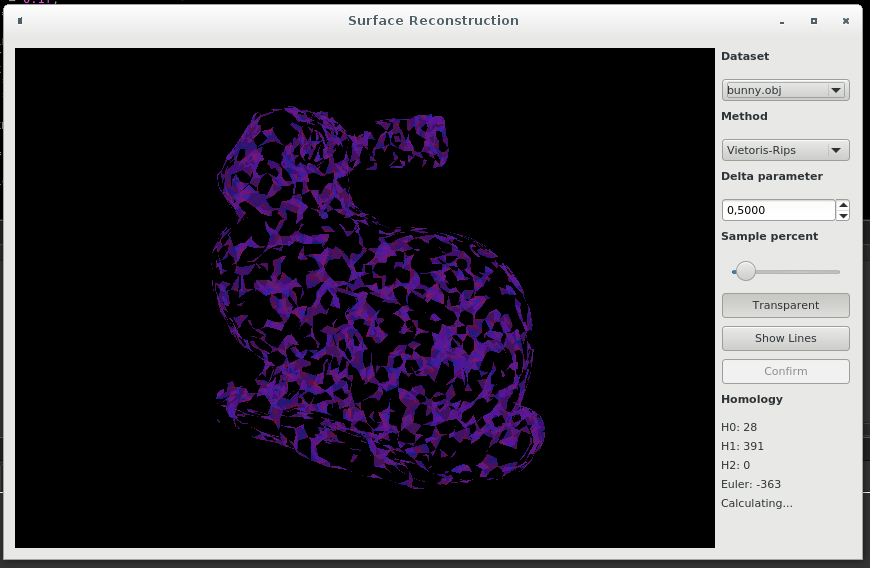
\includegraphics[width=0.6\textwidth]{vr_long.png}
    \caption{Izra"cun Viterbi-Ripsa s premajhnim delta.}
    \label{fig:vr1}
\end{figure}


\begin{figure}[htb]
    \centering
    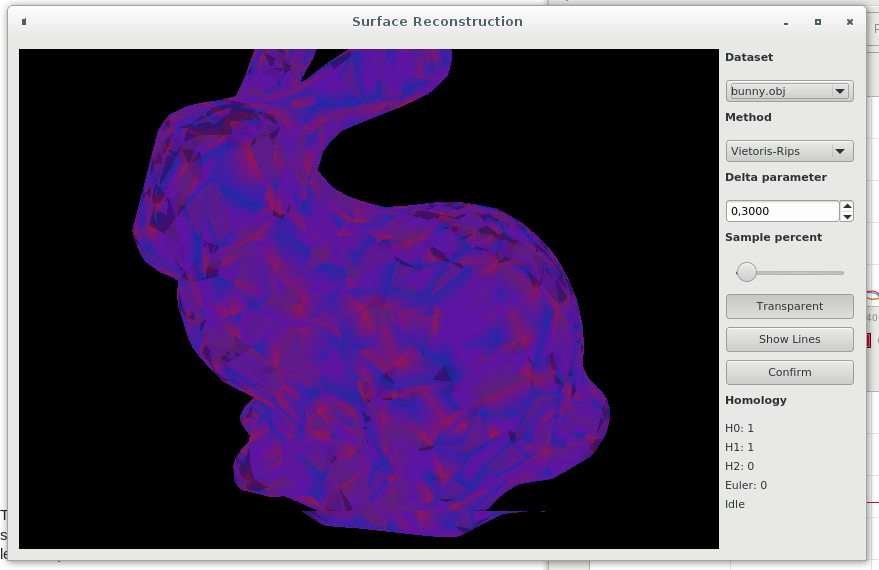
\includegraphics[width=0.6\textwidth]{vr_full_9639823.png}
    \caption{Izra"cun Viterbi-Ripsa z zadostnim delta, vendar malo to"ckami. "St. to"ck: 9639823}
    \label{fig:vr2}
\end{figure}

\begin{figure}[htb]
    \centering
    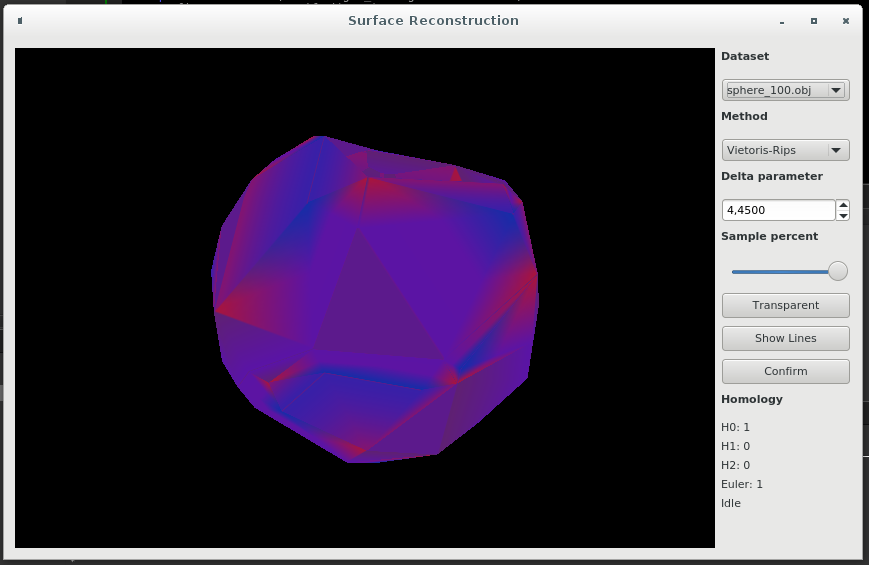
\includegraphics[width=0.6\textwidth]{vr_1hole.png}
    \caption{Izra"cun Viterbi-Ripsa n krogli: ena luknja}
    \label{fig:vr3}
\end{figure}

\begin{figure}[htb]
    \centering
    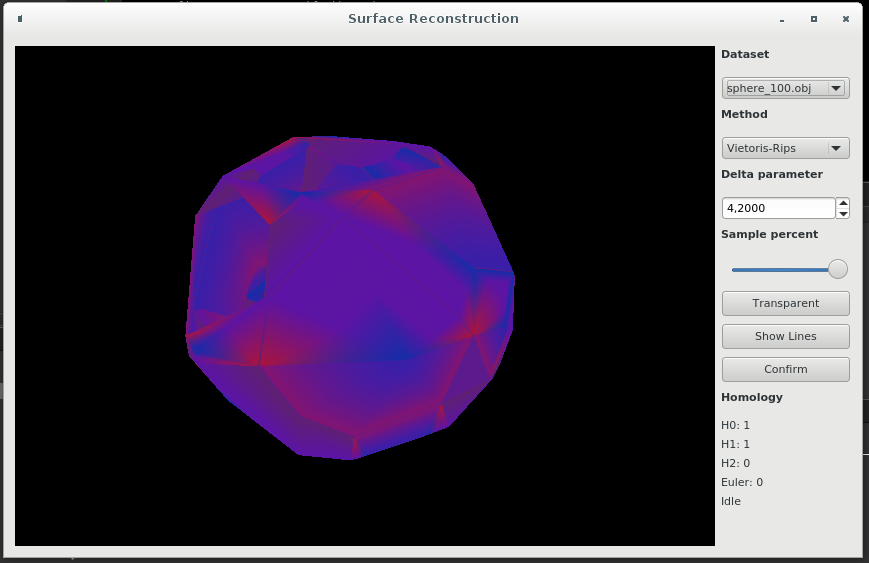
\includegraphics[width=0.6\textwidth]{vr_2hole.png}
    \caption{Izra"cun Viterbi-Ripsa n krogli: dve lunkji}
    \label{fig:vr4}
\end{figure}

\begin{figure}[htb]
    \centering
    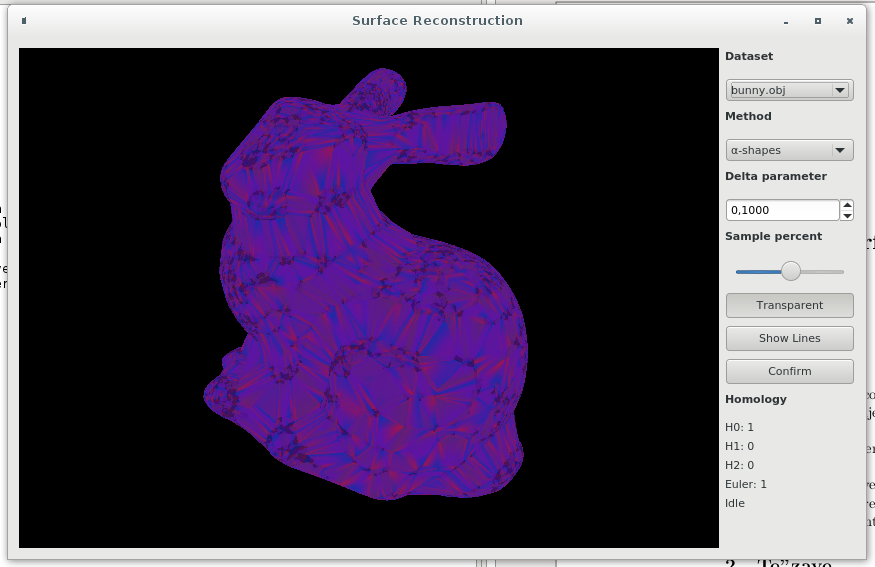
\includegraphics[width=0.6\textwidth]{alpha_full.png}
    \caption{Izra"cun $\alpha$ oblik: polno, ena lunkja na dnu zajca.}
    \label{fig:a1}
\end{figure}

\begin{figure}[htb]
    \centering
    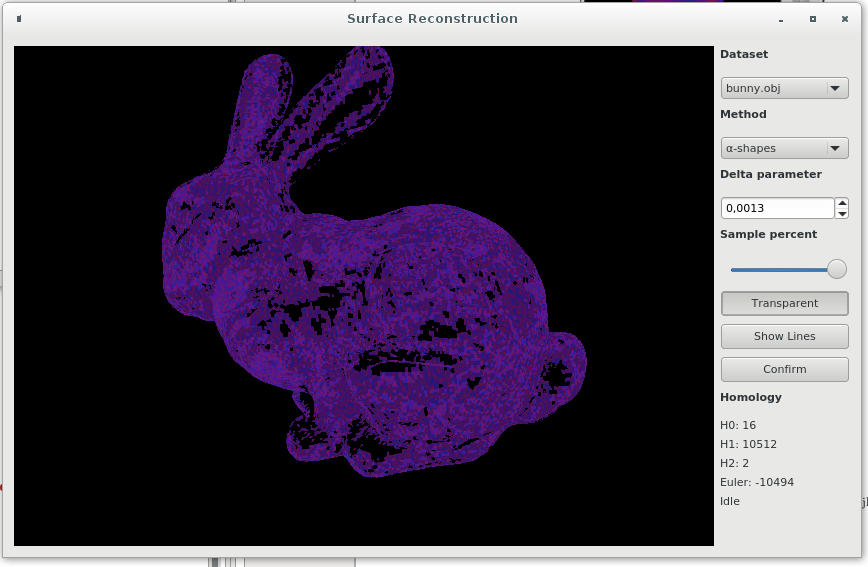
\includegraphics[width=0.6\textwidth]{alpha_lowdelta.png}
    \caption{Izra"cun $\alpha$ oblik: polno, Izra"cun na vseh to"ckah, a s premajhnim $\delta$}
    \label{fig:a1}
\end{figure}

\begin{figure}[htb]
    \centering
    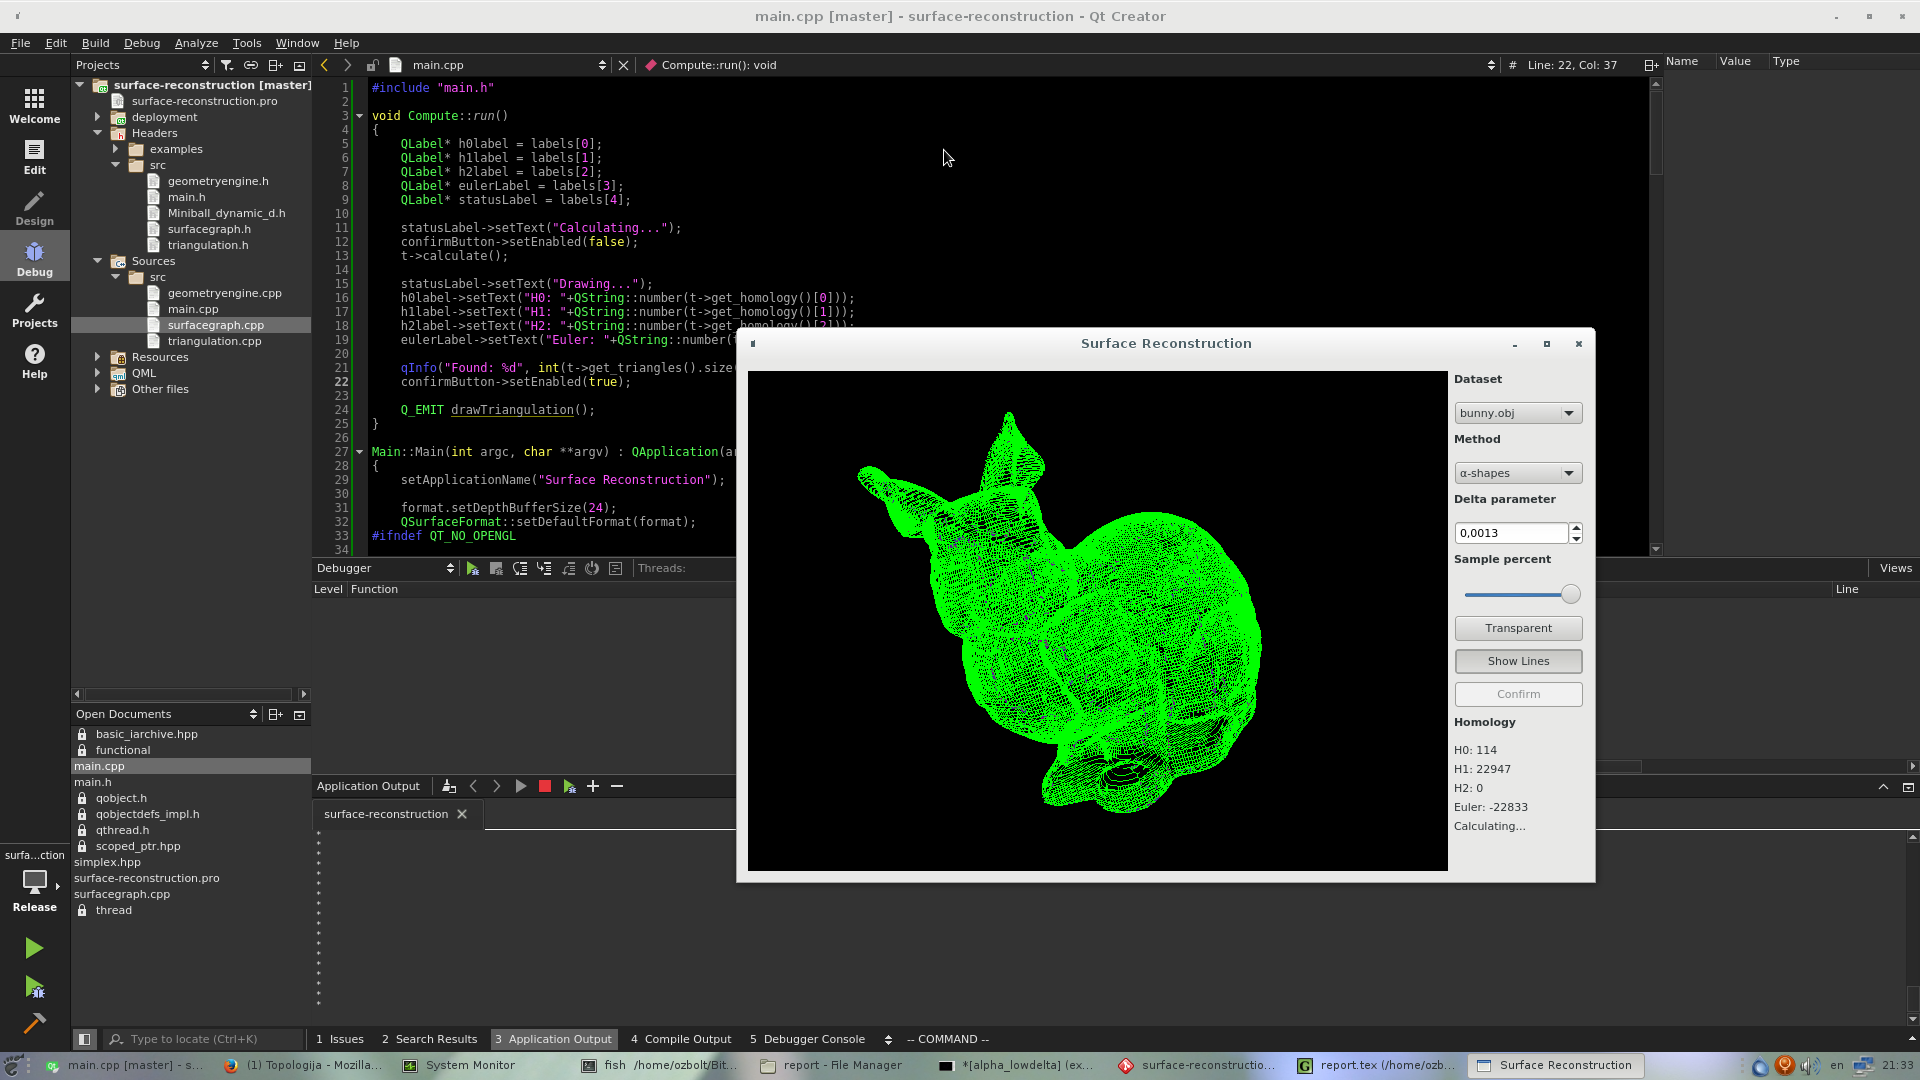
\includegraphics[width=\textwidth]{lines.png}
    \caption{Prikaz povezav.}
    \label{fig:edges}
\end{figure}

\end{document}
